\documentclass[12pt]{article}
\usepackage{amsmath}
\usepackage{hyperref}
\usepackage{verbatim}
\usepackage{graphicx}
\begin{document}
\subsection{Numerical Simulation Goals}\label{numergoals}
I will use the form of $\vec{B}$ given in Section \ref{subsecgenexam}, but I will have to make it divergentless, I will do this by introducing a radial field component in the trapping region:
\begin{equation}\label{magmirfield}
\vec{B}=B_0(1+z^2/L^2)\hat{z}-B_0(zr/L^2)\hat{r}
\end{equation}
This is divergentless if we operate in cylindrical coordinates. From here, we can use the Lorentz force law \eqref{lorenz} to generate the differential equations to solve (derived simply by carrying out the cross product with a generic velocity vector):
\begin{equation}\label{magmirDEs}
\begin{split}
\dot{v}_r=\frac{q}{m}v_{\theta}B_z\\
\dot{v}_{\theta}=\frac{q}{m}(B_rv_z-v_rB_z)\\
\dot{v}_z=-\frac{q}{m}B_rv_{\theta}
\end{split}
\end{equation}
The goal from here is to figure out initial conditions, and then solve the equations, and then plot them in the form of a movie.

I will be modifying the code presented in this \href{https://www.youtube.com/watch?v=d4NlmGkfagk&t=889s&ab_channel=PyPhy}{video}, and taking notes from \href{http://www.amazon.com/gp/product/0750310251/ref=as_li_ss_tl?ie=UTF8&tag=slovcook-20&linkCode=as2&camp=217145}{Birdsall's book}. 
\subsection{Boris Algorithm}
The particle equations of motion to be integrated are (assuming no force outside of electric and magnetic): 
$$\frac{d\textbf{v}}{dt}=\frac{q}{m}\left(\textbf{E}+\textbf{v}\wedge\textbf{B}\right)$$
$$\frac{d\textbf{x}}{dt}=\textbf{v}$$
We want a centered difference scheme, and we do this by evaluating the velocity vector at half-steps:
\begin{equation}\label{discretlorenz}
\frac{\textbf{v}_{t+\Delta t/2}-\textbf{v}_{t-\Delta t/2}}{\Delta t}=\frac{q}{m}\left(\textbf{E}+\frac{\textbf{v}_{t+\Delta t/2}+\textbf{v}_{t-\Delta t/2}}{2}\wedge\textbf{B}\right)
\end{equation}
The Boris algorithm introduces new velocity variables to separate the solution steps of the magnetic and electric fields:
\begin{equation}\label{v+v-}
\begin{split}
\textbf{v}^-=\textbf{v}_{t-\Delta t/2}+\frac{q\textbf{E}}{m}\frac{\Delta t}{2}\\
\textbf{v}^+=\textbf{v}_{t+\Delta t/2}-\frac{q\textbf{E}}{m}\frac{\Delta t}{2}
\end{split}
\end{equation}
Plugging this into \eqref{discretlorenz} yields
\begin{equation}\label{discretboris}
\frac{\textbf{v}^+-\textbf{v}^-}{\Delta t}=\frac{q}{2m}(\textbf{v}^++\textbf{v}^-)\wedge\textbf{B}
\end{equation}
This is a pure rotation of $\textbf{v}$. To show this, let's take the dot product of \eqref{discretboris} with $(\textbf{v}^++\textbf{v}^-)$, doing this cancels out the RHS because the dot product of perpendicular vectors is zeros, so we get
$$\textbf{v}^+\cdot(\textbf{v}^++\textbf{v}^-)=\textbf{v}^-\cdot(\textbf{v}^++\textbf{v}^-)$$
Taking advantage of the commutative nature of the dot product we get
$$|v^+|^2=|v^-|^2$$
Since $\textbf{v}^+$ is the time evolution of $\textbf{v}^-$ the only thing that \eqref{discretboris} can change is orientation, and thus it is only a rotation. Therefore, if we know what angle is traversed we can use rotation matrices in the solution process. In fact the solution process is the following:
\begin{itemize}
\item Add half the electric impulse to $\textbf{v}_{t-\Delta t/2}$ via \eqref{v+v-} to obtain $\textbf{v}^-$
\item Rotate through the angle dictated by \eqref{discretboris} to get $\textbf{v}^+$
\item Add the remaining half of the electric impulse to $\textbf{v}^+$ to obtain $\textbf{v}_{t+\Delta t/2}$
\end{itemize}
Now we need to derive the angle by which the velocity is rotated, we can do it by drawing the following figure:

\hspace{-2cm}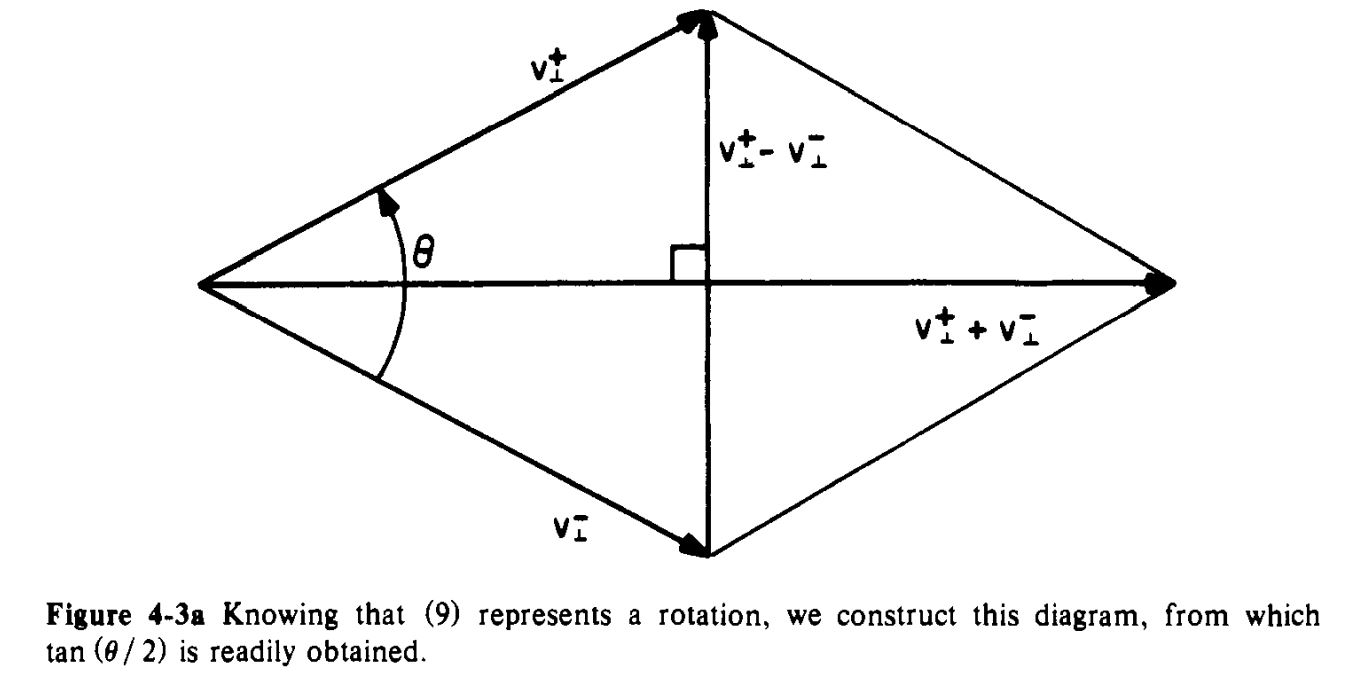
\includegraphics[scale=0.5]{anglerotated}
By construction, if we take half of $\textbf{v}^+_{\perp}-\textbf{v}^-_{\perp}$ and $\textbf{v}^+_{\perp}+\textbf{v}^-_{\perp}$ we get the legs of the right triangle in the upper left, and therefore:
$$tan\left(\frac{\theta}{2}\right)=\frac{|\textbf{v}^+_{\perp}-\textbf{v}^-_{\perp}|}{|\textbf{v}^+_{\perp}+\textbf{v}^-_{\perp}|}$$
We can then use \eqref{discretboris} and take the magnitude of the cross product with the components of the velocity perpendicular to $\textbf{B}$ and we get
$$\frac{|\textbf{v}^+_{\perp}-\textbf{v}^-_{\perp}|}{|\textbf{v}^+_{\perp}+\textbf{v}^-_{\perp}|}=\frac{qB\Delta t}{2m}$$
Therefore:
$$\bigg| tan\left(\frac{\theta}{2}\right)\bigg|=\frac{qB\Delta t}{2m}=\frac{\omega_c\Delta t}{2}$$
Now, by using the Lorenz force and the right hand rule, we realize that a particle gyrates with the opposite sign of the charge (if one defines counterclockwise as positive, as is customary), so we get a relative minus sign for $\theta$ and as $tan$ is an odd function we can define $t$ as
\begin{equation}\label{angleboris}
t\equiv tan\left(\frac{\theta}{2}\right)=-\frac{qB\Delta t}{2m}
\end{equation}
if we use the half angle formulas for $sin$ and $cos$ we get:
\begin{equation}\label{sandc}
\begin{split}
s\equiv -sin\theta =\frac{2t}{1+t^2}\\
c\equiv cos\theta=\frac{1-t^2}{1+t^2}
\end{split}
\end{equation}
Therefore, the rotation becomes
$$v_x^+=cv^-_x+sv^-_y$$
$$v_y^+=-sv^-_x+cv^-_y$$
We can reduce the number of multiplications involved in this system by defining a new variable:
\begin{equation}\label{Buneman}
\begin{split}
v_x'=v_x^-+v_y^-t\\
v_y^+=v_y^--v_x's\\
v_x^+=v'_x+v_y^+t
\end{split}
\end{equation} 
Boris (cite 1970 paper) generalized this to a case in which $\textbf{v}$ and $\textbf{B}$ have arbitrary directions via a cross product:
\begin{equation}\label{borisv'}
\textbf{v}'=\textbf{v}^-+\textbf{v}^-\wedge\textbf{t}
\end{equation}
By construction $\textbf{v}'$ is perpendicular to both $\textbf{B}$ and $\textbf{v}^+-\textbf{v}^+$, which means that the angle between $\textbf{v}^-$ and $\textbf{v}'$ is $\theta/2$, thus, we can draw the following figure:

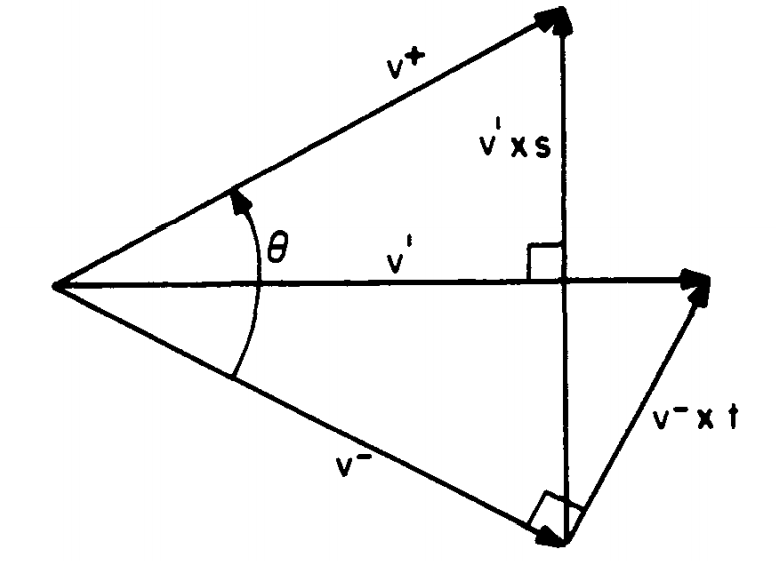
\includegraphics[scale=0.4]{vprimerot}

which shows us that 
\begin{equation}\label{tvec}
\textbf{t}\equiv-\hat{\textbf{b}}tan\left(\frac{\theta}{2}\right)=\frac{q\textbf{B}}{m}\frac{\Delta t}{2}
\end{equation}
As $\textbf{v}'$ is by construction perpendicular to both $\textbf{B}$ and $\textbf{v}^+-\textbf{v}^-$ and we are in a three-dimensional space, $\textbf{v}'\wedge\textbf{B}$ is parallel to $\textbf{v}^+-\textbf{v}^-$ and so if we define a vector $\textbf{s}$ which is parallel to $\textbf{B}$ we can make the statement:
\begin{equation}\label{borisv+}
\textbf{v}^+=\textbf{v}^-+\textbf{v}'\wedge\textbf{s}
\end{equation} 
If we take the dot product of each side we get
$$|v^+|^2=\textbf{v}^+\cdot\textbf{v}^-+\textbf{v}^+\cdot(\textbf{v}^-\wedge\textbf{s})+\textbf{v}^+\cdot(\textbf{v}^-\wedge\textbf{t})\wedge\textbf{s}$$
Let's look at just the triple product term:
$$(\textbf{v}^-\wedge\textbf{t})\wedge\textbf{s}=-\textbf{v}^-(ts)$$
Where $\textbf{v}^-\cdot\textbf{s}$ cancel because they are perpendicular. Which, when plugged into the above expression yields:
$$|v^+|^2=(1-ts)|v^-|^2cos\theta+\textbf{v}^+\cdot(\textbf{v}^-\wedge\textbf{s})=(1-ts)|v^-|^2\frac{1-t^2}{1+t^2}+\textbf{s}\cdot(\textbf{v}^+\wedge\textbf{v}^-)$$ 
Where I have used the identity derived earlier: $|v^+|^2=|v^-|^2$ as well as \eqref{sandc} and properties of the scalar product. As $\textbf{v}^+$ and $\textbf{v}^-$ form a plane, their cross product gives a vector antiparallel to $\textbf{s}$ by the right hand rule, therefore we get (again using \eqref{sandc})
$$|v^+|^2=(1-ts)|v^-|^2\frac{1-t^2}{1+t^2}-s|v^-|^2sin\theta=(1-ts)|v^-|^2\frac{1-t^2}{1+t^2}+s|v^-|^2\frac{2t}{1+t^2}$$
Pulling out a common factor:
$$|v^+|^2=|v^-|^2\frac{(1-ts)(1-t^2)+2st}{1+t^2}$$
By the fact that we want $|v^+|^2=|v^-|^2$
$$1+t^2=1+ts-t^2+st^3$$
$$2t=(1+t^2)s$$
And since $\textbf{s}$ is definitionally parallel to $\textbf{B}$ we get
\begin{equation}\label{boriss}
\textbf{s}=\frac{2\textbf{t}}{1+t^2}
\end{equation}
Finally, we can combine \eqref{v+v-}, \eqref{borisv'}, \eqref{tvec}, \eqref{borisv+}, and \eqref{boriss} to get the full Boris algorithm for the Lorenz force with no additional forces:
\begin{equation}\label{borisalgorithm}
\begin{split}
\textbf{t}\equiv-\hat{\textbf{b}}tan\left(\frac{\theta}{2}\right)=\frac{q\textbf{B}}{m}\frac{\Delta t}{2}\\
\textbf{s}=\frac{2\textbf{t}}{1+t^2}\\
\textbf{v}^-=\textbf{v}_{t-\Delta t/2}+\frac{q\textbf{E}}{m}\frac{\Delta t}{2}\\
\textbf{v}'=\textbf{v}^-+\textbf{v}^-\wedge\textbf{t}\\
\textbf{v}^+=\textbf{v}^-+\textbf{v}'\wedge\textbf{s}\\
\textbf{v}_{t+\Delta t/2}=\textbf{v}^++\frac{q\textbf{E}}{m}\frac{\Delta t}{2}
\end{split}
\end{equation}
Of course, the goal of this algorithm is to find the evolution of the position of the particles over time, and there is some subtlety with that due to the half step notation of $\textbf{v}$. The main loop is run with $\textbf{x}$ leading $\textbf{v}$ by $\Delta t/2$. Hence, at the start, $\textbf{v}(0)$ is moved backwards to $\textbf{v}(-\Delta t/2)$ (due to $\textbf{v}_{t-\Delta t/2}=\textbf{v}(t-\Delta t/2)$ so the initial point used for velocity is $\textbf{v}_{0-\Delta t/2}=\textbf{v}(-\Delta t/2)$)by first applying a rotation through the angle $\Delta\theta=\omega_c\Delta t/2$ then applying a half acceleration using $-\Delta t/2$ based on $\textbf{E}(0)$ obtained from $\textbf{x}(0)$. Alternatively, we can start the main loop by progressing $\textbf{v}$ forward by a half step in a traditional euler form, an example of this in python is
\begin{verbatim}
for i in range(0, self.N):
            
   QM = self.Q[i]/self.M[i]
            
   self.Vx[i] += QM* (Ex[i] + Bz[i]* self.Vy[i] - By[i]* self.Vz[i])* self.dt /2
   self.Vy[i] += QM* (Ey[i] + Bx[i]* self.Vz[i] - Bz[i]* self.Vx[i])* self.dt /2
   self.Vz[i] += QM* (Ez[i] + By[i]* self.Vx[i] - Bx[i]* self.Vy[i])* self.dt /2
\end{verbatim}
These can be treated as $\textbf{v}_{\Delta t/2}$ in 
$$\textbf{x}_1=\textbf{x}_0+\Delta t\textbf{v}_{\Delta t/2}$$
The above equation can be derived from centering the first derivative of $\textbf{x}$ at the half step:
\begin{equation}\label{finitevel}
\frac{\textbf{x}_{t+\Delta t}-\textbf{x}_t}{\Delta t}=\textbf{v}_{t+\Delta t/2}
\end{equation}
This is an example of a leapfrog method, with its characteristic half-step evaluations. Although the Boris algorithm as a whole is not a leapfrog method because of the fact that a leapfrog scheme cannot have the acceleration force depend on velocity (cite PPPL Boris letter), it is worth learning more about the leapfrog scheme as it describes the half-step evaluations for velocity while position is at a full step.
\subsection{Leapfrog Scheme}
For this section, I will begin by taking notes from this \href{https://en.wikipedia.org/wiki/Leapfrog_integration}{Wikipedia page}. 

A leapfrog method is one which is used to integrate systems of the following form:
$$\frac{dv}{dt}=A(x)$$
$$\frac{dx}{dt}=v$$
These differential equations are discretized in a centered scheme such that the velocity is evaluated at half steps and the position is evaluated at whole steps. The integrated progresses by interweaving position and velocity in a "leapfrog" pattern. Note that the derivative of velocity cannot depend on velocity to be considered a "leapfrog" method and come with all of the method's inherent advantages. Which includes the fact that it is symplectic in nature, which means that it conserves the (slightly modified) energy of dynamical systems.

Further notes on this subject will be taken from these \href{physics.ucsc.edu/~peter/242/leapfrog.pdf}{lectures}.

When looking at the slope of a chord between two points on a function, we find that it is a much better approximation of the derivative at the midpoint than at either end. For differential equations of a single degree of freedom (ie. where $\frac{dx}{dt}$ does not involve $x$, and $\frac{dv}{dt}$ does not involve $v$):
$$\frac{dx}{dt}=v$$
$$\frac{dv}{dt}=F(x)=-\frac{dU(x)}{dx}$$
The Euler method would integrate the first DE via $x_1=x_0+hv_0$, but a better approximation (second order) would be evaluating at the midpoint of $v$: $x_1=x_0+hv_{1/2}$, and so doing something similar for the velocity equation: $v_{3/2}=v_{1/2}+hF(x_1)$. From here, we can repeat the cycle, letting $x$ and $v$ leapfrog over each other after starting at the point $x_0$, $v_{1/2}$ for the increased accuracy. How accurate is this approach? Well, $x_1-x_0$ is of order $h$, for the midpoint approximation the leading error of $~h^2$ vanishes so the error for one interval is $h^3$. To integrate for a finite time $T$ the number of intervals is $T/h$ and so the overall error is proportional to $h^2$ and the leapfrog method is a second order method.

To make the leapfrog useful, however, two questions have to addressed: first, how do we start at $v_{1/2}$, since we only know $x_0$ and $v_0$? The simplest approximation is just to do a single half step of Euler: $v_{1/2}=v_0+\frac{1}{2}hF(x_0)$. Although this is not a midpoint method and has an order of $h$, we only do this once, so it does not lower the order of the method, which remains second order. The second question is how get the velocity at the same time as the position, which is needed to produce "phase space" plots and to compute the energy and angular momentum. The simplest approach is to consider $v_{n+3/2}=v_{n+1/2}+hF(x_{n+1})$ to be made up of two equal half steps, which successively relates $v_{n+1}$ to $v_{n+1/2}$ and $v_{n+3/2}$ to $v_{n+1}$. The leapfrog algorithm with a means of starting the algorithm and determining $x$ and $v$ at the same times is called velocity Verlet. A single time step can be written as
$$v_{n+1/2}=v_n+\frac{1}{2}hF(x_n)$$
$$x_{n+1}=x_n+hv_{n+1/2}$$
$$v_{n+1}=v_{n+1/2}+\frac{1}{2}hF(x_{n+1})$$
This is the same as the leapfrog method because we have just separated $v_{n+3/2}=v_{n+1/2}+hF(x_{n+1})$ into two steps. We could also do it so that we start with a half step of position followed by a full step of velocity followed by a half step of velocity.

There are several advantages to this algorithm, one of them is that the method is time reversible. It conserves angular momentum exactly. The leapfrog algorithm is "symplectic" ie area preserving. To better understand this, consider a small rectangular region of phase space of area $dA$. Let the four corners of the square, $(x,p),(x+dx,p),(x,p+dp),(x+dx,p+dp)$ represent four possible coordinates of a particle at time t. These are labeled 1,2,3,4. Then , at a later time $t'$ each of thse four points will have changed, to form the corners of a parallelogram. Let the area of the parallelogram be $dA'$. An important theorem (Liouville's theorem) states that the areas are equal: $dA=dA'$. $(x,p)$ transforms to $(x',p')$ where $x'$ and $p'$ are some functions of x, and p:
$$x'=X(x,p)$$
$$p'=P(x,p)$$
A set of equations like this, in which values of one set of variable is transformed to new values, is called a map. Thus, the result of integration of Newton's laws by a finite amount of time can be represented as an area preserving map. Since the area preserving property is an exact feature of the equations, it is desirable that a numerical approximation preserve it. Such approximations are called $\textit{symplectic}$. What is the condition for a map to be symplectic? To see this we need to compute the area $dA'$, and set it equal to $dA=dxdp$. The area $dA'$ is given by 
$$dA'=|d\vec{e}_1'\wedge d\vec{e}_2'|$$
Where $d\vec{e}_1'$ and $d\vec{e}_2'$ are the vectors describing the two sides of the parallelogram. Now, the components of $d\vec{e}_1'$ are just the changes in $x'$ and $p'$ when x is changed by $dx$ put $p$ is fixed, ie:
$$d\vec{e}_1'=\left(\frac{\partial x'}{\partial x}\hat{x}+\frac{\partial p'}{\partial x}\hat{p}\right)dx$$
and similarly
$$d\vec{e}_2'=\left(\frac{\partial x'}{\partial p}\hat{x}+\frac{\partial p'}{\partial p}\hat{p}\right)dp$$
The vector product representing $dA'$ can be represented by a determinant where we get
$$dA'=det JdA$$
where
$$J=\begin{bmatrix}
\frac{\partial x'}{\partial x} & \frac{\partial x'}{\partial p}\\
\frac{\partial p'}{\partial x} & \frac{\partial p'}{\partial p}
\end{bmatrix}$$
$det J$ is the Jacobian of the transformation from $(x',p')$ to $(x,p)$ which occurs when you change variables in an integral:
$$\iint\dots dx'dp'=\iint\dots detJ dx dp$$
Hence, a symplectic algorithm has $detJ=1$ to show that the leapfrog method is symplectic, we should consider each step of the Verlet algorithm separately. If we compare the first step at two nearby points: $(x_0,v_0)$ and $(x_0+\delta x_0,v_0+\delta v_0)$:
$$v_{1/2}+\delta v_{1/2}=v_0+\delta v_0+\frac{h}{2}F(x_0+\delta x_0),\hspace{5mm}v_{1/2}=v_0+\frac{h}{2}F(x_0)$$
Subtracting and letting $\delta x_0$ and $\delta v_0$ tend to zero, we get a matrix equation:
$$\begin{pmatrix}
\delta x_0\\
\delta v_{1/2}
\end{pmatrix}=A\begin{pmatrix}
\delta x_0\\
\delta v_0
\end{pmatrix}$$
Where
$$A=\begin{bmatrix}
1&0\\
\frac{h}{2}F'(x_0)&1
\end{bmatrix}$$
Using the other steps in the Verlet algorithm
$$\begin{pmatrix}
\delta x_1\\
\delta v_{1/2}
\end{pmatrix}=B\begin{pmatrix}
\delta x_0\\
\delta v_{1/2}
\end{pmatrix}\hspace{5mm}\begin{pmatrix}
\delta x_1\\
\delta v_1
\end{pmatrix}=C\begin{pmatrix}
\delta x_1\\
\delta v_{1/2}
\end{pmatrix}$$
Where
$$B=\begin{bmatrix}
1&h\\
0&1
\end{bmatrix}\hspace{5mm}C=\begin{bmatrix}
1&0\\
\frac{h}{2}F'(x_1)&1
\end{bmatrix}$$
Since the Jacobian is the evolution matrix of perturbations (a stretching matrix), we can write
$$\begin{pmatrix}
\delta x_1\\
\delta v_1
\end{pmatrix}=J\begin{pmatrix}
\delta x_0\\
\delta v_0
\end{pmatrix}$$
Where we know $J$ from the previous analysis: $J=CBA$, as the determinant of a product of matrices is the product of determinants of the individual matrices, and the determinants of $A$, $B$, and $C$ are all 1 by inspection
$$detJ=1$$
And the leapfrog is symplectic. The advantage of symplectic algorithms is that possess global stability. Since the area bounded by adjacent trajectories is preserved, we can never have the situation that the coordinates increase without bound, because this would expand the area. As well, the numerically calculated energy oscillates with small amplitude around the correct value, instead of diverging like the Euler method would. Note that the leapfrog algorithm is formulated for position dependent (conservative) forces only, and thus, it is not automatic that the Boris algorithm would have this symplectic property. The assumption that the force is velocity independent is because if this assumption is broken, the leapfrog method becomes implicit, and no long functional as originally formulated. A method for generic velocity dependent forces is the Taijama inversion method. This method is expensive, and so treated only as a last resort. 
\subsection{Boris Algorithm Properties}
The Boris algorithm posseses the long-time stability characteristic of a leapfrog method, despite having a velocity dependent force. This includes exact energy conservation when the electric field is zero, and bounded energy error when the electric field is non-zero (cite PPPL report). As well, the Boris algorithm has been found to solve for a particle's trajectory accurately for an arbitrarily large number of steps (cite). It as well is phase-space volume preserving. 
\subsection{Learning the Sample Code}
I will follow through the video series examples in order to learn the code. The following examples are from this \href{https://www.youtube.com/watch?v=UC5gy7bhAns&t=70s&ab_channel=PyPhy}{video}
\begin{itemize}
\item Example 1:
What is the motion of positive and negative particles in a magnetic field?

In the inputs.txt file we will set
\begin{verbatim}
N    = 1
tmax = 7
dt   = 1E-3
\end{verbatim}
Then in the Initial.py code we will set
\begin{verbatim}
self.x,  self.y,  self.z  = [0], [0], [0]
self.Vx, self.Vy, self.Vz = [1], [0], [0]
self.M,  self.Q           = [1], [1]
\end{verbatim}
in the innit function in the MakeDataFiles class. We will run the Initial code. In the Main.py file, we will set 
\begin{verbatim}
def B(self):
        
        Bx, By, Bz = [0]* self.N, [0]* self.N, [0]* self.N
        
        # Case - 1 : Constant B field
        Bz = [1]* self.N
\end{verbatim}
Which gives a B-field of 1 Tesla in the z-direction, and zero Tesla everywhere else. We will then run Main.py. At the top of the PlotData.py file I added 
\begin{verbatim}
from mpl_toolkits.mplot3d import Axes3D
from IPython import get_ipython
\end{verbatim}
This allows me to do a 3D plot in a different window. I set the potential to zero, and I plotted the data which gives:

\hspace{-1cm}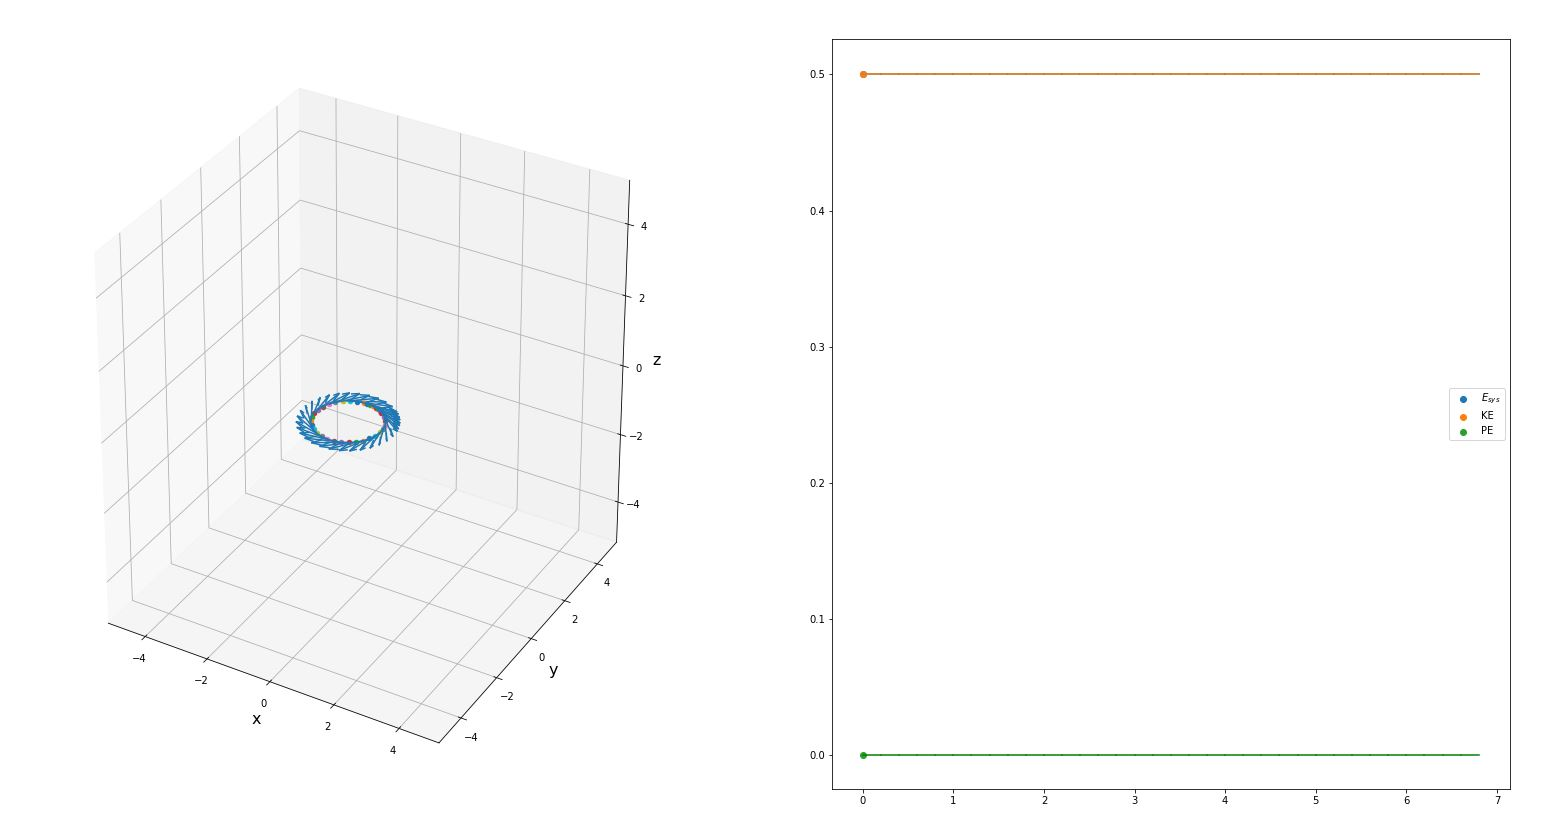
\includegraphics[scale=0.35]{example1}

Which matches theory well. However, as can be seen, the proportions of the produced graphs are much too small, and as such, that is something I will fix when I modify this code. However, I can zoom into the 3D plot to get a better view:

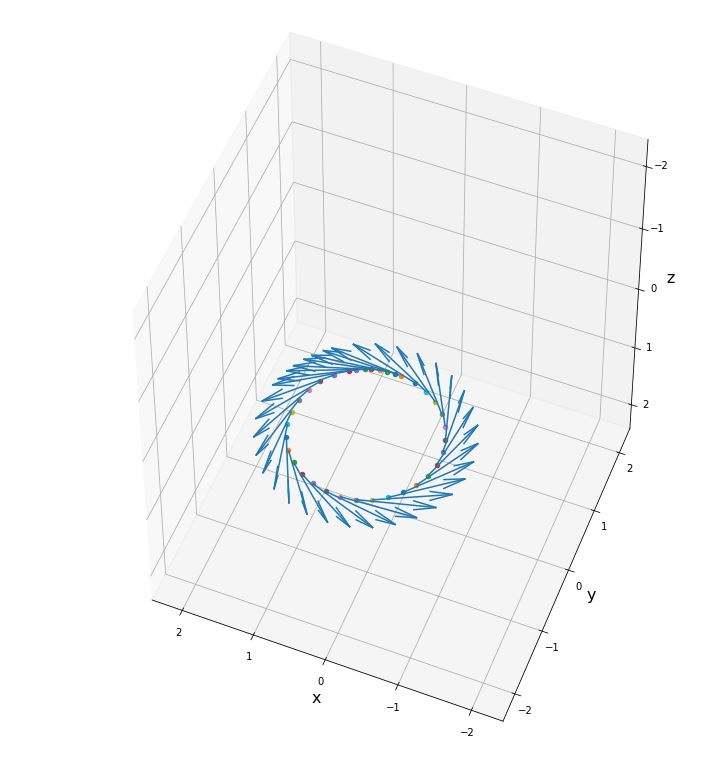
\includegraphics[scale=0.4]{example1,2}

Note that the energy values are constant, so it is clear that the magnetic field is doing no work, which again, agrees with theory.

\item Example 2: Add velocity parallel to the magnetic field line to the previous problem

We do this by changing the Initial.py to:
\begin{verbatim}
self.x,  self.y,  self.z  = [0], [0], [-2]
self.Vx, self.Vy, self.Vz = [2], [0], [0.5]
self.M,  self.Q           = [1], [1]
\end{verbatim}
Running the other two codes again gives:

\hspace{-1cm}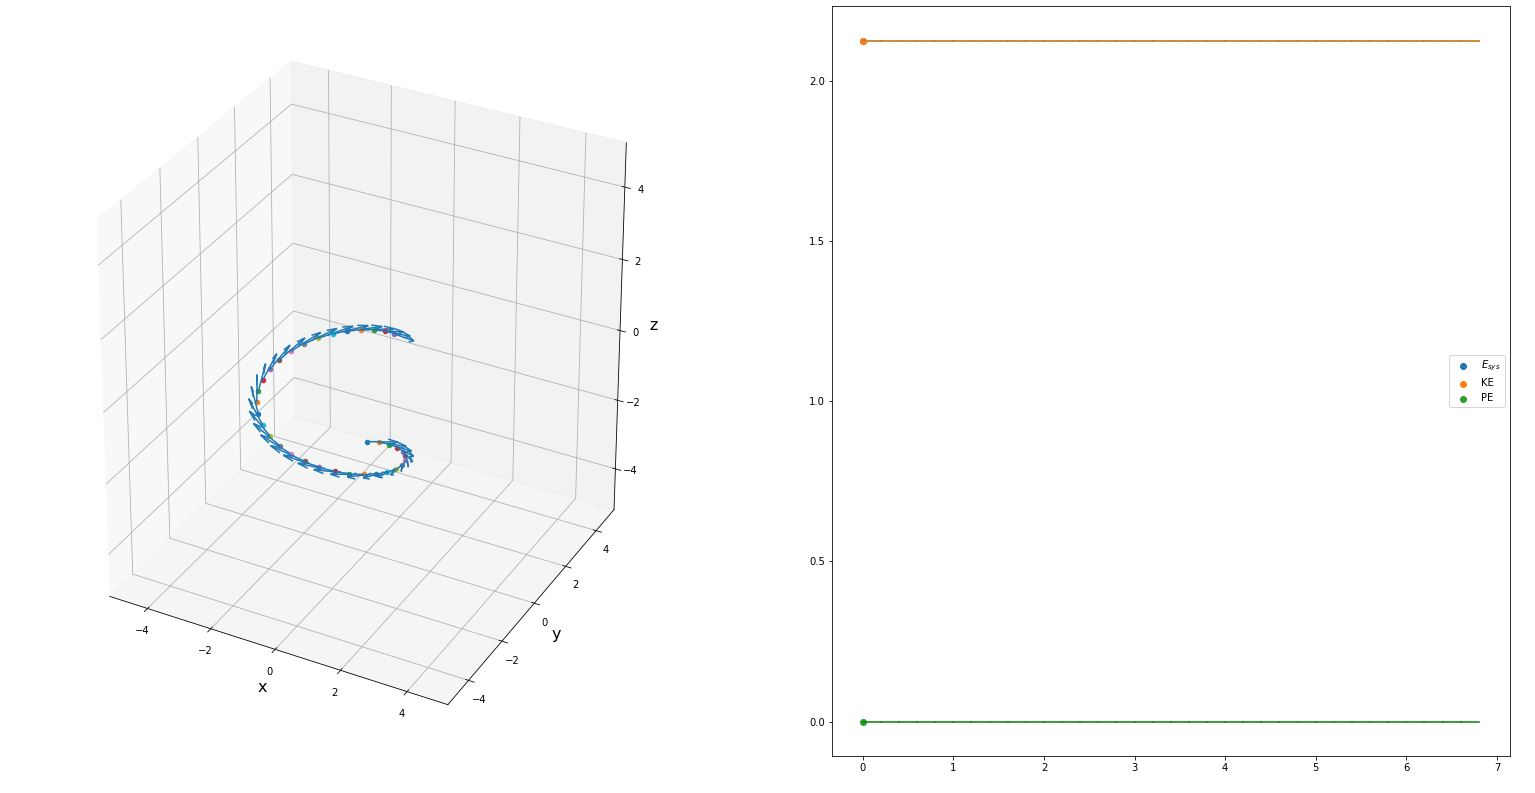
\includegraphics[scale=0.35]{example2}

\item Example 3: Constant Electric and Magnetic Fields

Adds a drift velocity of the form $v_{\vec{E}\wedge\vec{B}}=\frac{\vec{E}\wedge\vec{B}}{B^2}$ which is independent of charge. We model this by changing tmax in Inputs.txt to 20. And in Initial.py we change the initial conditions:
\begin{verbatim}
self.x,  self.y,  self.z  = [0], [0], [0]
self.Vx, self.Vy, self.Vz = [1], [1], [0]
self.M,  self.Q           = [1], [1]
\end{verbatim}
Then we can add the constant Electric field in Main.py, and add the external force potential due to the work the Electric field does:
\begin{verbatim}
for i in range(0, self.N):
             Ex[i] += 1
             Ey[i] += 0
             Ez[i] += 0
\end{verbatim}
This yields

\hspace{-1cm}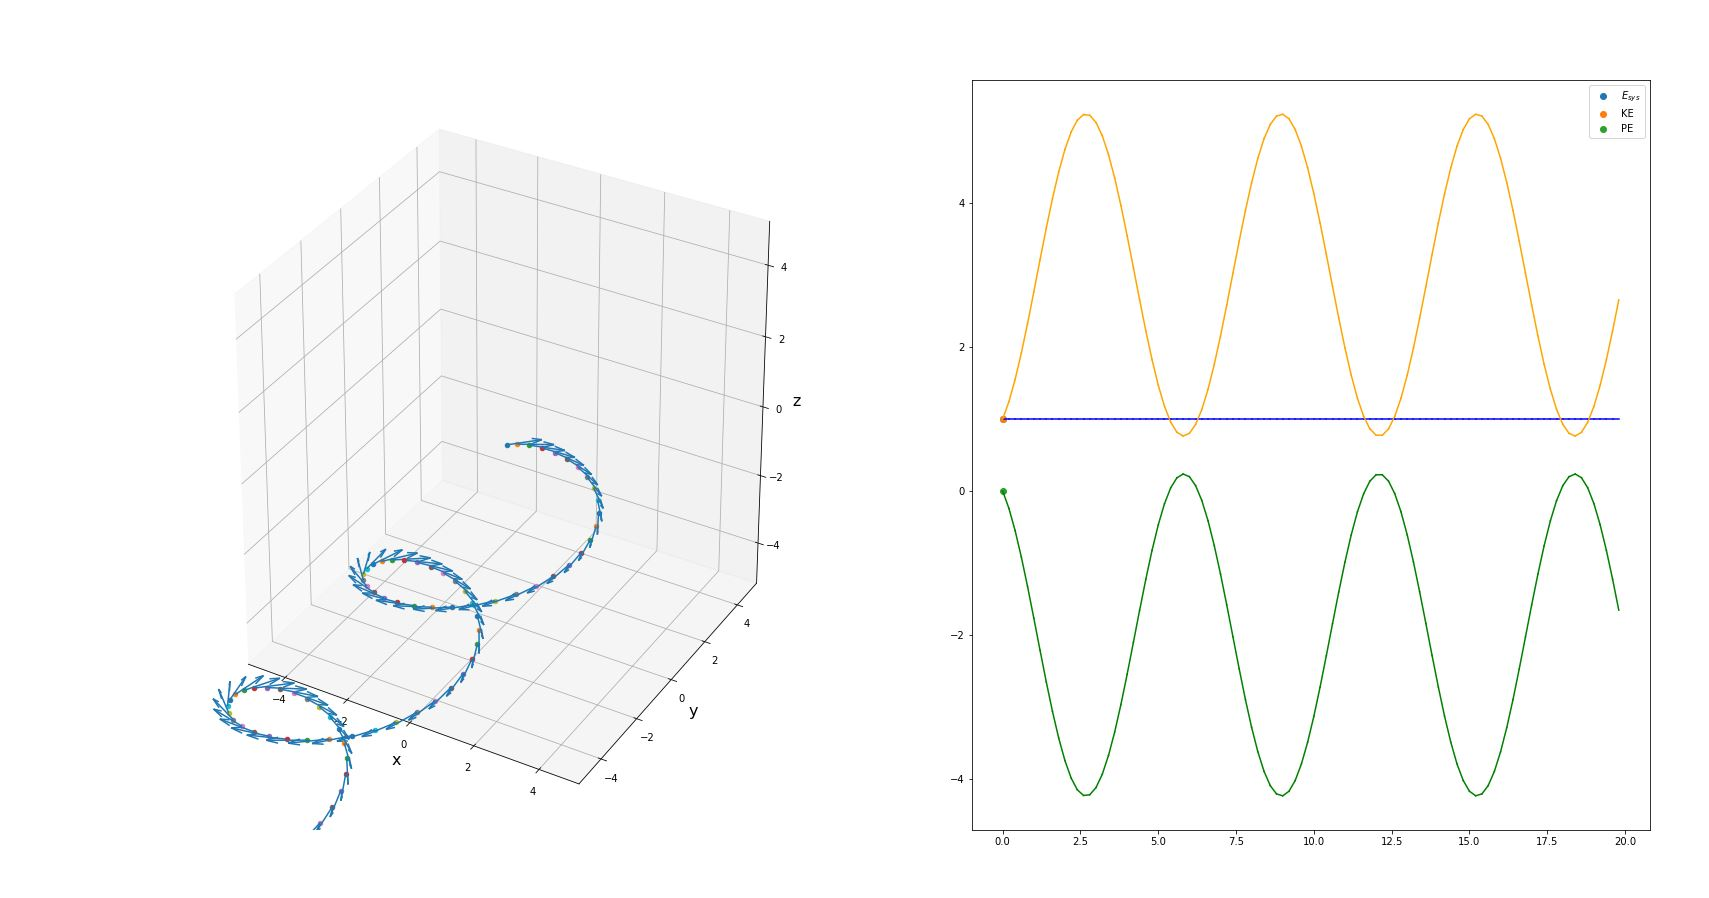
\includegraphics[scale=0.35]{example3}
\end{itemize}
I can also do a basic magnetic mirror, but I'll talk about that more in the next section.
\subsection{Numerical Simulation of a Magnetic Mirror}
Finally, it is time to modify the sample code to work for the problem in Section \ref{subsecgenexam}. First, I want to add to the above sample code, the ability to automatically assign end points to the plot. Specifically, for the magnetic mirror without gravity, I want to add the turning points calculated early in the General's Problem:
\begin{equation}\label{nogravturnpts}
z_T^2=\frac{W_{\parallel0}}{W_{\perp0}}L^2
\end{equation}
This will give an immediate visual check of my work in Section \ref{subsecgenexam}. However, we must first numerically define $W_{\parallel0}=\frac{1}{2}mv_{\parallel0}^2$ and $W_{\perp0}=\frac{1}{2}mv_{\perp0}^2$. The easiest way to do this is to apply Gram-Schmidt with the intention of producing two basis vectors: one parallel to the magnetic field, one perpendicular. The following formulae are courtesy of Tal Rubin:
\begin{equation}\label{paraperpvelocities}
\begin{split}
\vec{v}_{\parallel}=\frac{\vec{v}\cdot\vec{B}}{B^2}\vec{B}\\
\vec{v}_{\perp}=\vec{v}-\frac{\vec{v}\cdot\vec{B}}{B^2}\vec{B}
\end{split}
\end{equation}
Then we can just find the magnitude squared of each of these vectors evaluated at the midplane, and plug them into the equations for $W_{\parallel0}$ and $W_{\perp0}$. I will initially write my code with the assumption that the particle starts at the midplane, so  $z=0$. So in the code I will set
\begin{verbatim}
self.x,  self.y,  self.z  = [0], [0], [0]
\end{verbatim} 
This means that the magnetic field in Section \ref{numergoals} becomes $\vec{B}=B_0\hat{z}$. For both parallel and perpendicular energy, we need to find the magnitude squared of the parallel and perpendicular velocities:
\begin{equation}\label{paraperpmags}
\begin{split}
v_{\parallel}^2=\frac{(\vec{v}\cdot\vec{B})^2}{B^2}\\
v_{\perp}^2=v^2-\frac{(\vec{v}\cdot\vec{B})^2}{B^2}
\end{split}
\end{equation}
This was just calculated by taking dot products of \eqref{paraperpvelocities} of the equations with themselves. If we evaluate both $\vec{v}$ and $\vec{B}$ at the midplane we can calculate $W_{\parallel0}$ and $W_{\perp0}$. If we assume the particle(s) start at the midplane, we need to use the values of velocity before they are progressed forward a half step. I integrate this into the code by adding the following into the main Boris algorithm function:
\begin{verbatim}
#parallel kinetic energy            
WP0 = 0
for i in range(0, self.N):
   WP0 += self.M[i]*0.5*(self.Vx[i]*Bx[i]+self.Vy[i]*By[i]+self.Vz[i]*Bz[i])**2/
   (Bx[i]**2+By[i]**2+Bz[i]**2) 
        
#perpendicular kinetic energy
WPerp0=0
for i in range(0,self.N):
   WPerp0=self.M[i]*0.5*(self.Vx[i]**2+self.Vy[i]**2+self.Vz[i]**2
   -(self.Vx[i]*Bx[i]+self.Vy[i]*By[i]+self.Vz[i]*Bz[i])**2/
   (Bx[i]**2+By[i]**2+Bz[i]**2))
\end{verbatim} 
Note that this was place in the initialization step of the Boris algorithm, so right before the half-step of velocity is calculated, and right after the function which defines the B-field is called. The dot products are fully written out here to fit with the formatting of the sample code, later I will rewrite so that Python carries out the dot product symbolically. I also added a line of code which writes the above calculation into a txt file and stores it so that another program may access it (namely the sample program which does the plotting). However, this is not all we need to add, currently, the sample code does not place an upper bound on the size of the mirror machine. So, all particles are trapped because they can just keep traveling until the magnetic field gets strong enough to repel them. This is obviously not what we need to model Section \ref{subsecgenexam}. To address this, I add the argument L to the Boris function, and then in the loop which loops through each particle I add:
\begin{verbatim}
if (self.z[i]>=L) or (self.z[i]<=-L):
   print('escaped')
   escaped +=1
\end{verbatim}
Then, in the while loop which terminates after a certain time is reached, I added an if statement which breaks the loop if more than half the particles have escaped:
\begin{verbatim}
if escaped > self.N/2:
   break
\end{verbatim}
I hope to keep this code working for more than one particle, despite my current lack of knowledge on how a magnetic mirror works with more than one particle. Finally, I need to modify the function which creates the magnetic field to match \eqref{magmirfield}. I also need to adjust the initial conditions so that the particle doesn't escape. I choose
\begin{verbatim}
self.x,  self.y,  self.z  = [0], [0], [0]
self.Vx, self.Vy, self.Vz = [1], [0], [0.25]
self.M,  self.Q           = [1], [1]
\end{verbatim}
In this circumstance, $\vec{B}$ is only along the z-direction so any velocity not in that direction is perpendicular velocity. As well from Section \ref{subsecgenexam} we know that without gravity the trapping condition is
$$W_{\parallel0}\leq W_{\perp0}(R-1)$$
Where $R$ is the ratio of the minimum $B$ to maximum $B$, for this current simulation I set $R$ as close to 2 as the radial component would allow. When taking into account the radial component, the definition of $R$ becomes
$$R\equiv\frac{\sqrt{B_z^2(max)+B_r^2(max)}}{B_0}$$
Since $B_r$ is dependent on $r$ there is some difficulty in calculating the exact $R$ value. However, when the charge to mass ratio of the simulated particles are realistic (for example a heavy proton, or an electron), the gyroradius of the particle is so small that $B_r$ is almost negligible, and so for my purposes I will use:
\begin{equation}\label{approxR}
R\approx\frac{B_z(max)}{B_0}
\end{equation}
This $R$ is slightly smaller than the real $R$, so the borderline predictions from the trapping conditions derived in Section \ref{subsecgenexam} are not valid, but the turning point predictions are pretty good, and the general trapping is quite accurate.

To determine the appropriate timestep, I ran simulations using $1E-03,1E-06,1E-07$ and $1E-08$. I found that $1E-07$ gave reasonable enough run times, and still gave smooth curves for the $x$ and $y$ positions. I used the $x$ and $y$ positions as benchmarks, because the charge to mass ratio I used (the value for a proton divided by 100) yields the fasted oscillations in the simulation. Therefore, if I choose a timestep which can accurately resolve this behavior, it is a timestep that can accurately resolve the whole system's behavior. For the length I set, I was aiming for an $R$ value of about 2. From Section \ref{subsecgenexam} we have a prediction of the turning points as
$$z_T=\pm\sqrt{\frac{W_{\parallel0}}{W_{\perp0}}}L$$
For the initial conditions I set, the length of the system, as well as the R value I approximated, this value should be $\pm 0.5$, the numerically calculated value is $0.4994286$ which less than a 0.2\% error. I can account for this by the fact that the prediction for the turning points assumes no radial contribution from the magnetic field, so even the small amount that exists due to gyromotion yields noticeable differences. The following are plots with a half length of 1, and an approximate $R=2$ with timestep $1E-07$ (the first being the x position versus time, and the second being the z position versus time): 
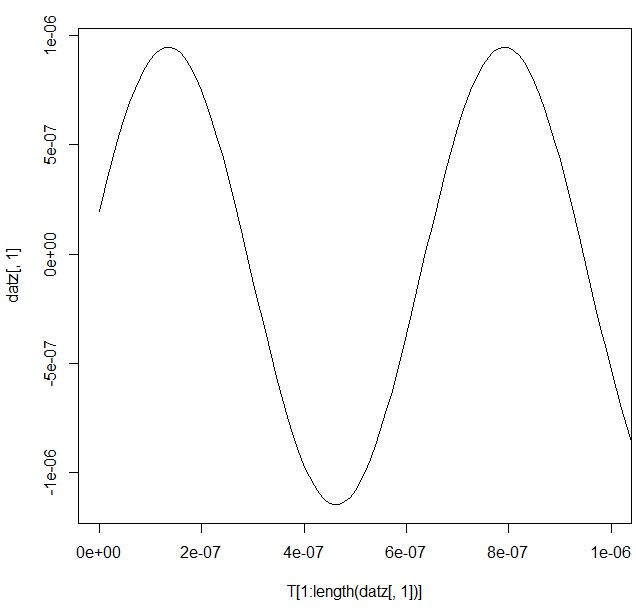
\includegraphics[scale=0.6]{xvt(L=1,R=2)}

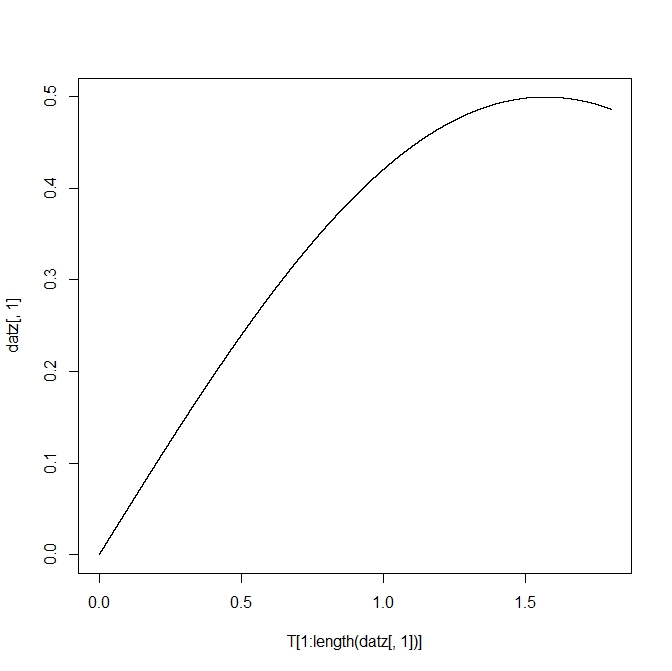
\includegraphics[scale=0.4]{zvt(L=1,R=2)}

As can be seen, the gyroradius is very small, as expected, and the oscillations are smooth, which can be seen with the following plot using just data points:

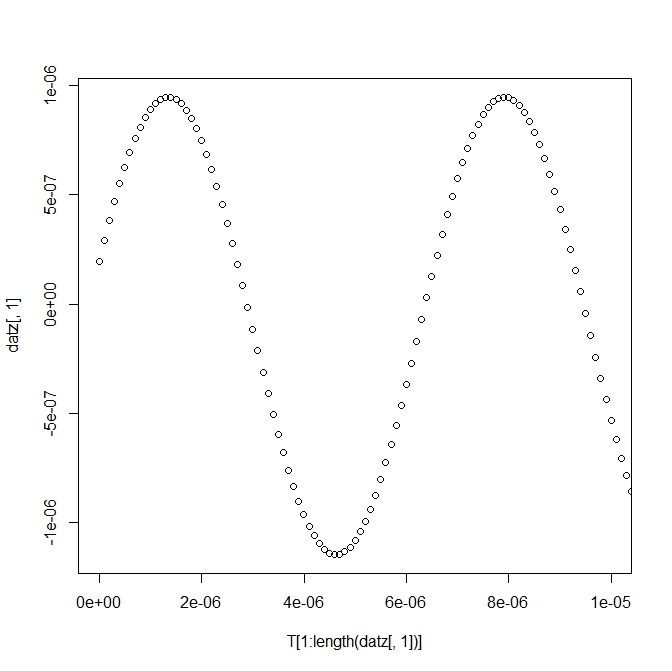
\includegraphics[scale=0.4]{xvtp(L=1,R=2)}

So our timestep is small enough. For quicker run times, I will be working with a mirror machine of half-length $0.1$, in this case, the turning point should be $0.05$, and the result is $0.04994286$ which, again, has less than a 0.2\% error, which, again, is very very good. So, that leads me to the conclusion, that using the approximate $R$ value is appropriate.

\subsection{Additions to the Code}
One goal of my project is to introduce asymmetries into the magnetic mirror. This was done in Section \ref{subsecgenexam} by adding a gravity field, this will be addressed as a generic velocity-independent force. In addition to non-E\&M forces, by adding a correctly calibrated electric field, we can induce rotation in the confined plasma.  
\subsubsection{$\vec{E}\wedge\vec{B}$ Drift}
Before we try to add rotation to our system, we need to understand $\vec{E}\wedge\vec{B}$ drift. If we add an electric field to the system which is perpendicular to the magnetic field it will accelerate particles traveling on their gyro orbits. This prevents the orbits from closing because at somepoint in the orbit the particle will be fighting the $E$-field, and at another point, it will be being pushed by it. This yields a drift perpendicular to the magnetic field, as orbiting through the electric field accelerates and decelerates an equal amount, if we average over the gyro-orbit the overall acceleration is zero, an so we can write
$$\vec{0}=\vec{E}+\vec{v}_{E\wedge B}\wedge\vec{B}$$
If we take the lefthanded cross product of $\vec{B}$ on either side of the equation we obtain
$$\vec{0}=\vec{B}\wedge\vec{E}+\vec{B}\wedge\vec{v}_{E\wedge B}\wedge\vec{B}$$
We can then use the vector triple product, and the fact that $\vec{v}_{E\wedge B}$ is perpendicular to $\vec{B}$ to obtain
\begin{equation}\label{EcrossB}
\vec{v}_{E\wedge B}=\frac{\vec{E}\wedge\vec{B}}{B^2}
\end{equation} 
For our purposes, we want $\vec{E}\perp\vec{B}$, so we can find the magnitude of the drift velocity to be
\begin{equation}\label{driftmag}
v_{E\wedge B}=\frac{E}{B}
\end{equation} 
Of course, normally, we look at drifts in Cartesian coordinates, so the drift just goes off in a straight line, but in cylindrical coordinates, it is possible to isolate the $\hat{\theta}$ basis vector, and thus produce a rotational plasma. But how do we do this? First, we see that the direction of the drift is dictated by $\vec{E}\wedge\vec{B}$, so we must force this cross product to be only in the $\hat{\theta}$ direction, or else particles will leave the system. This can be accomplished by ensuring that the $E$-field does not have a $\hat{\theta}$ component, as the $B$-field for a magnetic mirror only has $\hat{r}$ and $\hat{z}$ components, this yields a cross product of $(B_rE_z-E_rB_z)\hat{\theta}$, so that answers the directional question. However, we want the electric field to be perpendicular to the magnetic field so that we can get predictable results. This can be accomplished systematically by taking a dot product of the two fields and setting it to zero, which yields:
\begin{equation}\label{radialE}
E_r=-\frac{B_z}{B_r}E_z
\end{equation}
As an electric field is already built into the Boris algorithm, all we need to do to implement this is to define the electric field according to \eqref{radialE}.
\subsubsection{Generic Velocity-Independent Force} 
In Section \ref{subsecgenexam} a gravitational field was introduced into the mirror. This exerts a special force on the particle, which is velocity independent. As this is the case, we can simply redefine \eqref{v+v-} to account for additional velocity independent forces:
\begin{equation}\label{v+v-gen}
\begin{split}
\textbf{v}^-=\textbf{v}_{t-\Delta t/2}+\frac{q\textbf{E}}{m}\frac{\Delta t}{2}+\textbf{F}\frac{\Delta t}{2m}\\
\textbf{v}^+=\textbf{v}_{t+\Delta t/2}-\frac{q\textbf{E}}{m}\frac{\Delta t}{2}-\textbf{F}\frac{\Delta t}{2m}
\end{split}
\end{equation}
This maintains the form of the Lorenz equation for the Boris algorithm \eqref{discretboris}, and so has all of its properties, and thus we just need to appropriately modify \eqref{borisalgorithm}, to simulate systems under the influence of these types of forces. To add this to the code I add
\begin{verbatim}
def F(self):
   Fx, Fy, Fz = [0]* self.N, [0]* self.N, [0]* self.N
        
   # Gravitational Field
   for i in range(0,self.N):
      Fx[i] += 0
      Fy[i] += 0
      Fz[i] += -self.M[i]*9.81
        
   return Fx, Fy, Fz
\end{verbatim}
Right before the start of the Boris loop, then within the loop
\begin{verbatim}
Fx, Fy, Fz = self.F()

QM = self.Q[i]/self.M[i]
self.Vz[i] += (Fz[i]/self.M[i]+QM* (Ez[i] + By[i]* self.Vx[i] - Bx[i]* self.Vy[i]))* self.dt /2

qd[i] = (self.Q[i]* self.dt)/ (2* self.M[i])
Ux[i]   = self.Vx[i] + qd[i]* Ex[i]+self.dt/(2*self.M[i])*Fx[i]
Uy[i]   = self.Vy[i] + qd[i]* Ey[i]+self.dt/(2*self.M[i])*Fy[i]
Uz[i]   = self.Vz[i] + qd[i]* Ez[i]+self.dt/(2*self.M[i])*Fz[i]

self.Vx[i] = Ux_d[i] + qd[i]* Ex[i]+self.dt/(2*self.M[i])*Fx[i]
self.Vy[i] = Uy_d[i] + qd[i]* Ey[i]+self.dt/(2*self.M[i])*Fy[i]
self.Vz[i] = Uz_d[i] + qd[i]* Ez[i]+self.dt/(2*self.M[i])*Fz[i]
\end{verbatim}
Where the $[i]$ indicates looping over every particle. Looking back at Section \ref{subsecgenexam}, the particle I simulated without gravity will become detrapped, so I will change the initial x velocity to $\sqrt{2}$ and the z velocity to $0.15$. This satisfies the rearranged trapping condition $v_{\parallel0}\leq\sqrt{v_{\perp0}^2-2gL'}$, where I have set $L'$ to $0.1$. We can now check the turning points according to the formula
$$z_{L,H}=\frac{-z_g\pm\sqrt{z^2_g+4z_T^2}}{2}$$
Where $z_T$ has already been defined and $z_g \equiv mgL^2/W_{\perp 0}$, which for these initial conditions yield $z_g=0.0981$, and $z_T^2=\frac{(0.15)^2}{2}(0.1)^2$. Plugging this into the turning point equation gives us $z_H=0.0011336875887$ and $z_L=-0.0992336875887$, as calculated by Desmos. The numeric results are $z_H=0.001133644$ and $z_L=-0.09900957$ or less than 0.01\% error, and less than 0.3\% error respectively, again the approximate $R$ formulation appears valid. A visual depiction of the results:

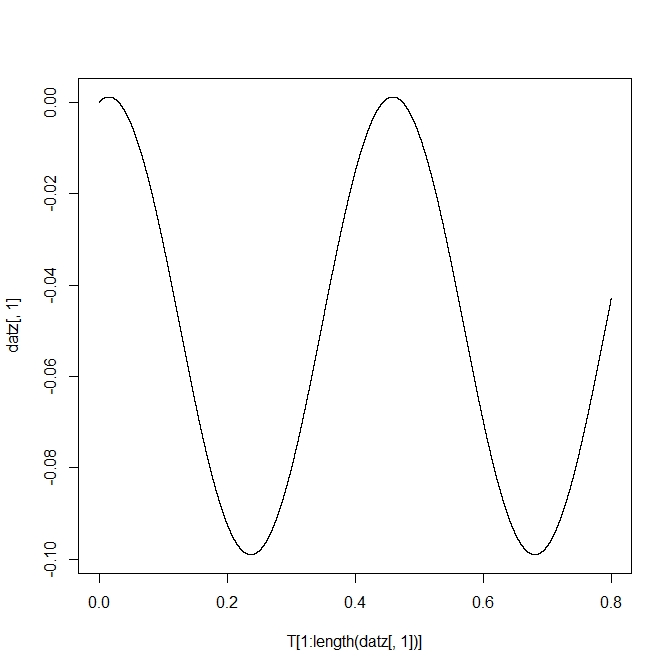
\includegraphics[scale=0.35]{zvtg(L=01,R=2)}

If we look at the point plot of the x-direction, we see that, again, a time step of $1E-07$ is low enough to maintain accuracy

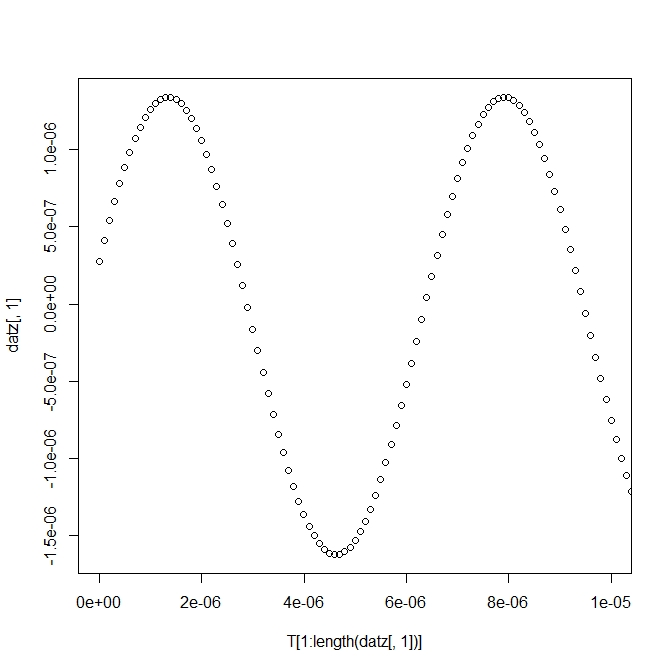
\includegraphics[scale=0.35]{xvtgp(L=01,R=2)} 

Finally, I want to check my answer for the last part of the generals problem. My answer was that a midplane parallel kinetic energy of zero, along with a midplane perpendicular kinetic energy of zero, are the two minimum values of initially trapped particles released as a gravitational potential is added over time. To do this, I first ran the simulation with no gravity and with a zero initial velocity, this remains trapped for the entire run time. Now, I will add linear dependence to the gravitational field: $g(t)=g*t/t_{final}$ so that the simulation starts at zero gravity, and ends at full gravity. I run the simulation again, including the time dependence. At a little over 45\% of the run time, the particle escaped, and thus because a position of $(0,0)$ on $W_{\perp0}-W_{\parallel0}$ space is the absolute smallest point, that has to be the smallest energies that start trapped, and become detrapped. 
\end{document}